\subsection{Predicted responses reveal relative spatial context sensitivity}
\label{sec:context-response}

Once a transformation predicts states at different observation ranges, their differences can be used to compare context dependence across locations. We evaluate the normalized response in Equation~\ref{eq:granularity-response} against directly encoded changes over the same intervals, with all predictions starting from a common $e_8$.

\paragraph{Predicted response orders context-sensitive locations.}
For each held-out section and each of four doubling intervals, we rank 1,024 locations by predicted response and compare the highest and lowest quarters. The high-response quarter has a larger mean directly encoded change in 31 of 32 section--interval conditions (Figure~\ref{fig:heldout-response-ordering}). Equal-section mean high-to-low ratios range from 1.440 to 1.673 across the four intervals. Predicted response thus identifies relative differences in how strongly tissue descriptions depend on observation range (Appendix~\ref{app:response-meaning}).

\begin{figure}[!htbp]
\centering
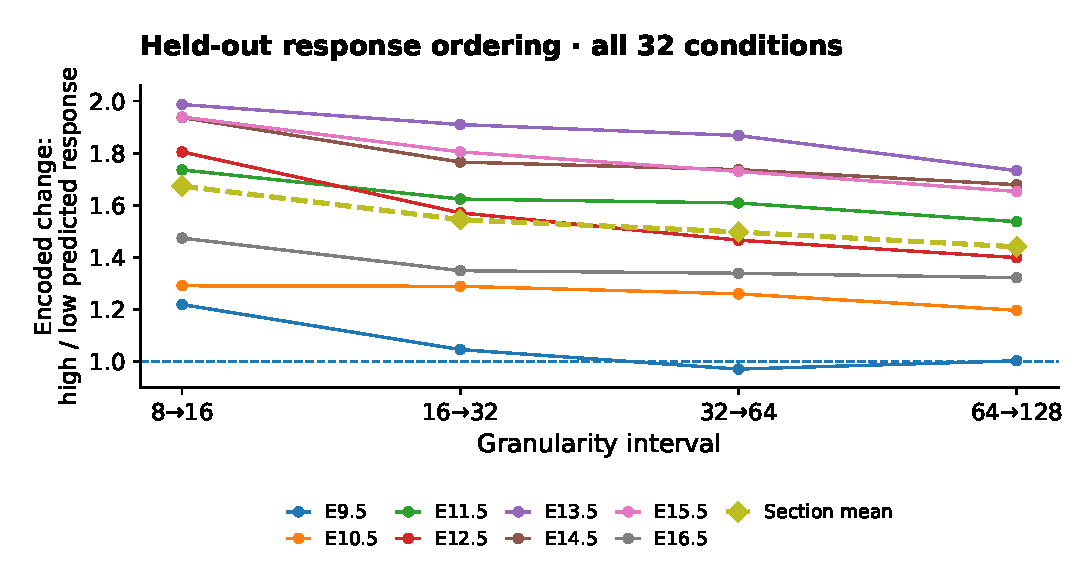
\includegraphics[width=0.78\linewidth]{figures/results_response_ordering.pdf}
\caption{\textbf{Predicted response identifies larger encoded changes on held-out sections.} Locations are ranked separately within each section and interval by predicted finite response. The ordinate is the ratio of mean directly encoded change in the highest versus lowest predicted-response quarter, with 256 locations per group. All 32 section--interval conditions are shown; 31 are above one. Lines denote sections and diamonds denote equal-section means. Full values: Table~\ref{tab:ode-response-heldout}.}
\label{fig:heldout-response-ordering}
\end{figure}

\paragraph{Anatomical context gives the response an interpretation.}
Two source-section cases illustrate distinct forms of context dependence. In E14.5 E1S1 Facial nerve, predicted and directly encoded changes correlate over $64\to128$ across all 64 locations ($\rho=0.791$; Figure~\ref{fig:scale-continuum}C). Predicted response also correlates with changes in annotated neighbor composition ($\rho=0.707$; Figure~\ref{fig:ode-context}A). In the highest-response quarter, the mean nerve fraction falls from 71.4\% to 45.7\% as context expands, compared with 43.4\% to 36.2\% in the lowest quarter (Figure~\ref{fig:ode-context}B). High-response locations therefore undergo a larger transition from a nerve-dominated neighborhood to surrounding tissue; low-response locations already include substantial surrounding tissue at the smaller range.

In E16.5 E1S1 Brain, context can change even when a broad annotation does not. Over $8\to16$, 95 sampled locations have only Brain-labeled neighbors at both granularities, yet their predicted and directly encoded responses correlate at $\rho=0.645$ (Appendix~\ref{app:response-meaning}). The response therefore captures molecular-context variation within a broad anatomical label as well as shifts in tissue composition. Whole-section maps illustrate the spatial heterogeneity of this dependence (Figure~\ref{fig:ode-context}C,D).

\begin{figure}[H]
\centering
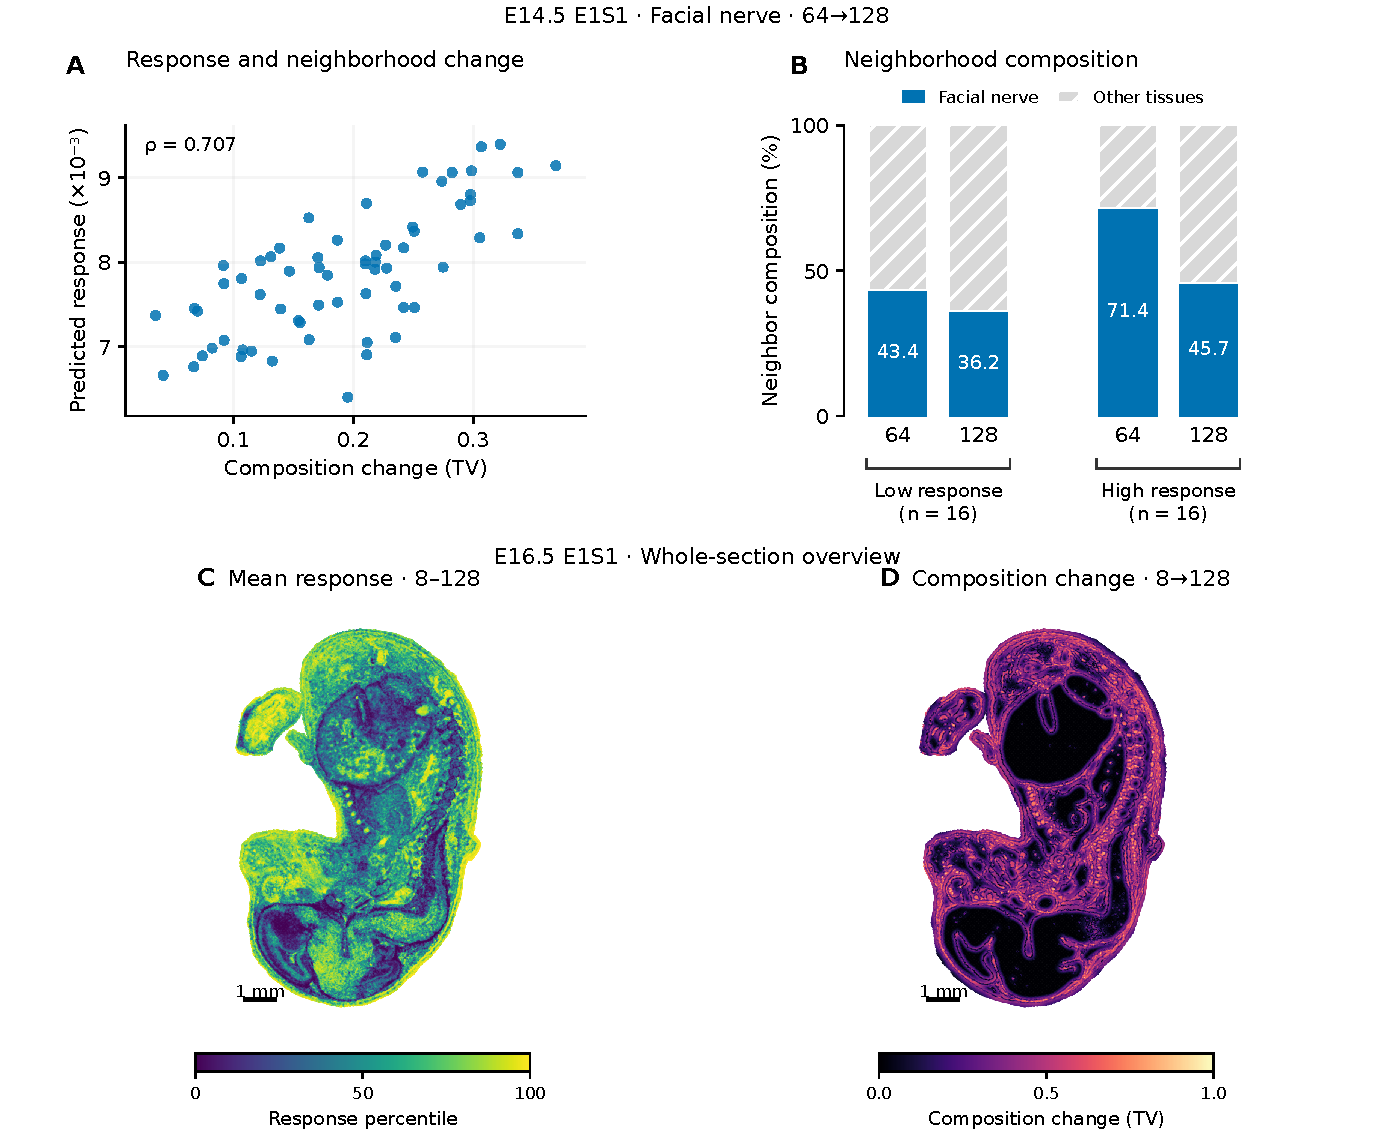
\includegraphics[width=0.92\linewidth]{figures/response_and_neighborhood_context.pdf}
\caption{\textbf{Context response distinguishes different dependencies on surrounding tissue.} \textbf{A}, Predicted finite response versus annotation-composition change (total variation, TV) at all 64 E14.5 E1S1 Facial nerve locations over $64\to128$. \textbf{B}, Mean composition at 64 and 128 for the lowest and highest response quarters, following the same 16 locations per group. \textbf{C,D}, E16.5 E1S1 whole-section maps of path-averaged instantaneous response over 8--128 (percentiles) and observed composition change from 8 to 128. These are spatial overviews of different quantities. All 121,767 locations are retained without smoothing. Both sections are anatomical cases from the training set; predictions start from fixed $e_8$. Scale bars: 1\,mm. Definitions: Appendix~\ref{app:response-meaning}.}
\label{fig:ode-context}
\end{figure}
